\chapter{Introduction}
\label{chapter_intro}

In this chapter we give a brief overview of cross site scripting (XSS), which is one of the most
common web application vulnerabilities. We mainly focus on DOM based XSS for which Trusted Types are
the most effective. We then explain the design of Trusted Types and how it helps to detect and
mitigate these vulnerabilities. Lastly, we describe the motivation and background for our work.

\section{Cross site scripting}

Cross site scripting (XSS) is one of the most prevalent vulnerabilities on the web. It is an attack
of web applications taking untrusted user input and interpreting it as code without sanitization or
escaping. There are multiple categories of XSS. Most experts distinguish at least between
non persistent \emph{(reflected)} and persistent \emph{(stored)} XSS. There is also a third
category, DOM based XSS, which will be explained in more depth as this is the threat model
under which Trusted Types operate.

\begin{itemize}
  \item  Stored -- A malicious injected script is permanently saved in a server database. The client
        browser will then ask the server for the requested page and the response from the server
        will contain the malicious script.
  \item  Reflected -- Typically delivered via email or a neutral website. It occurs when a
        malicious script is reflected off of a web application to the victim's browser
        \cite{reflected_xss}.
  \item  DOM based -- The vulnerability appears in the DOM (\ref{def:dom}) by executing a malicious
        code. In reflected and stored XSS attacks you can see the vulnerability payload in the
        server response. However in a DOM based XSS, the attack payload is executed as a result of
        modifying the DOM environment in the victim's browser so that the client side code runs in
        an unexpected manner.
\end{itemize}

Cross site scripting vulnerability became more widespread with the boom of single page applications
(SPA) (\ref{def:spa}), where most of the behaviour is achieved by modifying the DOM using
JavaScript. There are many functions, element attributes and properties in the DOM API which
interpret the arguments as an executable code. We call these DOM sinks (\ref{def:dom_source_sink}).
These sinks make it easy for developers to accidentally introduce this vulnerability
\cite{tt_web_framework_paper}.

\bigskip
\begin{lstlisting}[language={}, caption=Common DOM XSS sinks \cite{dom_xss_portswigger} \cite{tt_web_framework_paper}]
document.write()
element.innerHTML
element.insertAdjacentHTML
DomParser.parseFromString
frame.srcdoc
eval()
script.src
Worker()
\end{lstlisting}

\begin{figure}[H]
  \centerline{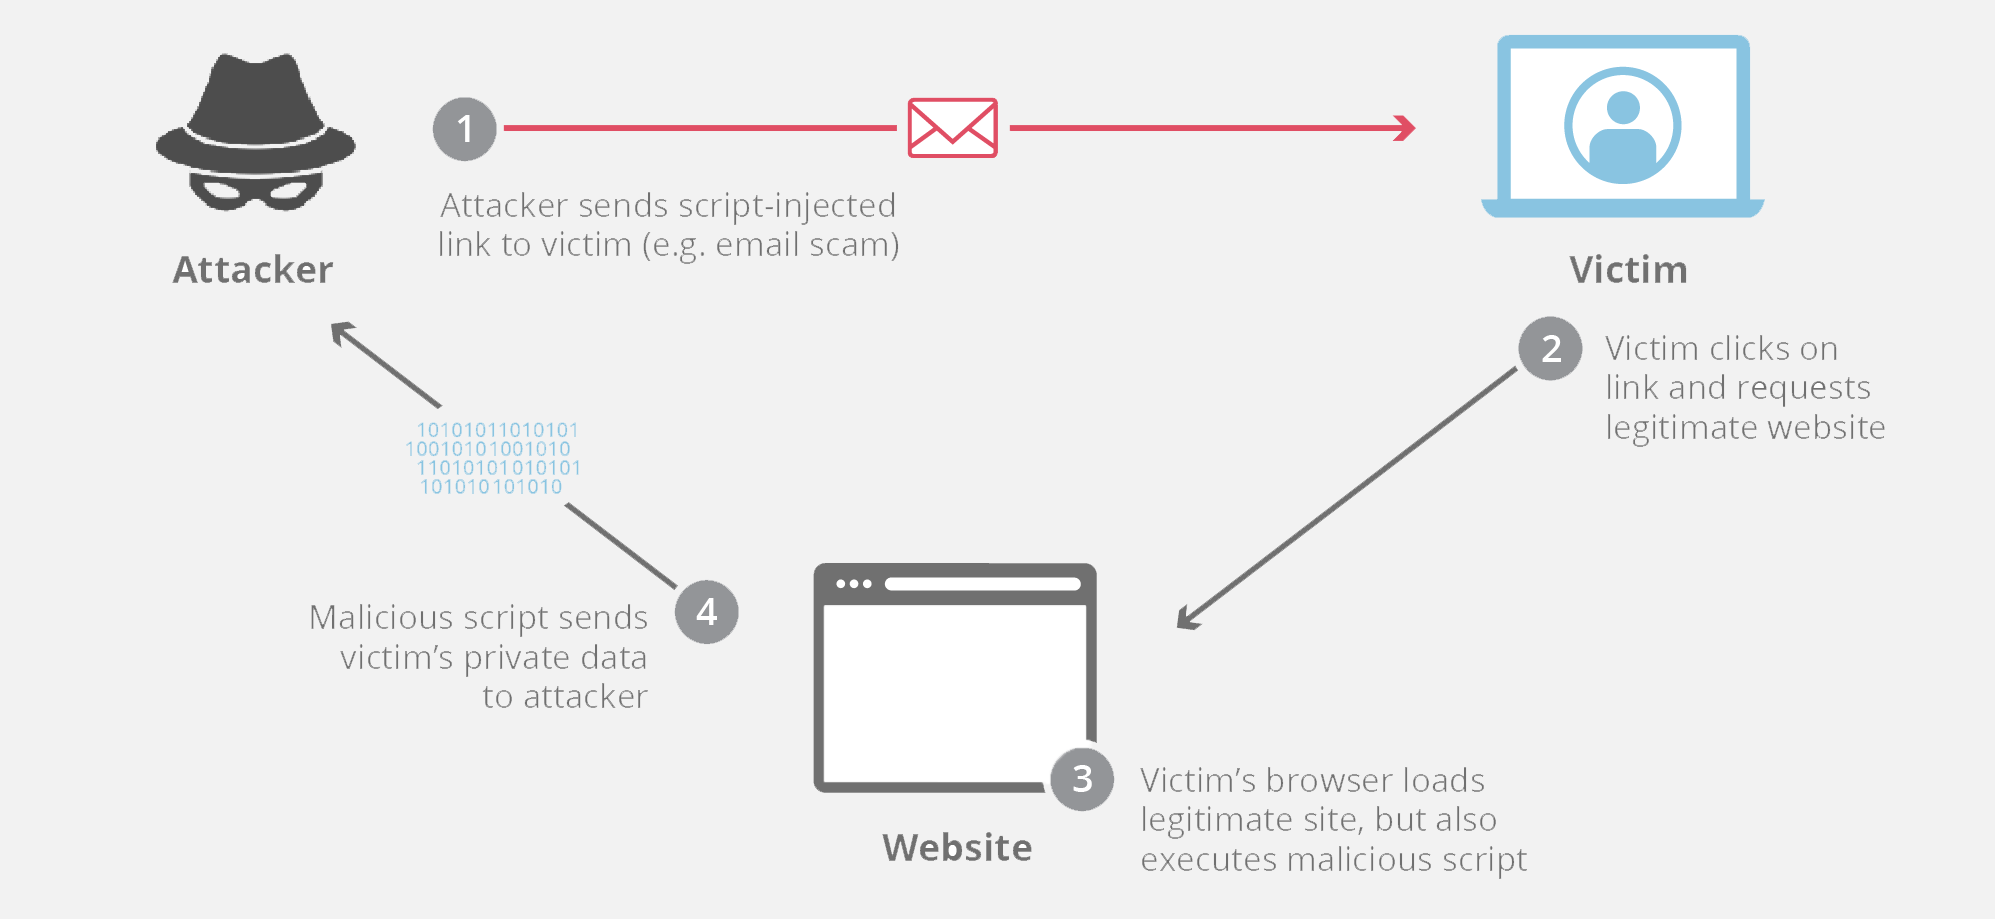
\includegraphics[width=1\textwidth]{images/xss-attack.png}}
  \caption[Common XSS vulnerability flow \cite{xss_image}]{Common XSS vulnerability flow \cite{xss_image}}
  \label{img:xss}
\end{figure}

One of the most basic examples of XSS is the interpolation of URL parameters in the DOM. The
attacker can prepare a malicious URL which he sends to a victim. The victim executes the payload
just by navigating to the site sent by the attacker.

\bigskip
\begin{lstlisting}[language=HTML, caption=Basic example of XSS via unsafe URL parameter interpolation]
<!--
Assume this page is on https://example.com.
It can be misused by the following attack payload:
https://example.com?<img%20src=x%20onerror="alert(1)"></img>
-->
<!DOCTYPE html>
<html lang="en">
  <body>
    <div id="content"></div>
    <script type="text/javascript">
      const content = decodeURIComponent(location.search.substr(1))
      document.getElementById('content').innerHTML = 'URL content: ' + content
    </script>
  </body>
</html>
\end{lstlisting}

The consequences of XSS vary a lot. Their severity can range from benign annoyances to unrecoverable
damages such as full account compromise, disclosure of user's cookies, storage, secrets or session.
Other attacks may use XSS to change the application content and present fraudulent information to the
user.

There are many attempts to reduce the risk of DOM XSS either by dynamic or static checkers. The
former usually suffer from performance and scalability issues when applied on large codebases while
the latter provide suboptimal results due to JavaScript dynamic nature
\cite{tt_web_framework_paper} \cite{owasp_xss_cheatsheet}.

\section{Trusted Types}

Trusted Types is a relatively modern web API designed by Google based on a long history of
mitigating XSS \cite{tt_design_history}.

It is a browser security feature that limits access to dangerous DOM APIs to protect against DOM
XSS. Trusted Types provide type guarantees to all frontend code by enforcing security type checks
directly in the web browser. They are delivered through a CSP header and have a report only mode
that does not change the application behavior and an enforcement mode that may cause user observable
breakages \cite{tt_background}.

When enforced, Trusted Types block dangerous injection sinks from being called with values that have
not passed through a Trusted Types policy \cite{tt_background}. If an untrusted value is passed to
sink a Trusted Types violation is raised and the DOM is unaffected. In practice this means that a
potential DOM XSS has been prevented.

There are many other resources which can be used to explore Trusted Types in details
\cite{tt_resources}.

\subsection{Threat model}

Trusted Types is a powerful API. Its main goals are to \cite{tt_spec:goals}:

\begin{itemize}
  \item reduce the risk of client side vulnerabilities caused by injection sinks.
  \item replace the insecure by default APIs with safer alternatives which are harder to misuse.
  \item encourage a design where the code affecting the application security is encapsulated in a
        small part of an application.
  \item reduce the security review surface for applications and libraries.
\end{itemize}

The main idea behind Trusted Types is to make the dangerous DOM APIs secure by default and encourage
application authors to use safer APIs. This model is very effective for preventing DOM based XSS,
however there are still areas where Trusted Types are not effective enough and other security
measures are needed. Some of the non goals of Trusted Types are \cite{tt_spec:non_goals}:

\begin{itemize}
  \item preventing or mitigating server side generated markup attacks -- Defending against XSS on
        both client and server can be really complex, especially for applications where parts of the
        code can run on both client and server, for example as in Next.js (\ref{intro-nextjs}). To
        address these attacks, use the existing recommended solutions like templating systems or CSP
        \emph{script-src}.
  \item controling subresource loading -- Trusted Types deal with code running in realm of the
        current document and does not guard subresources.
  \item guarding cross origin JavaScript execution, for example loading new documents via
        \emph{data:} URLs -- Trusted Types do not guard cross origin executions at all
  \item protecting against malicious developers of the web application -- It is implicitly assumed
        that untrusted developer can cause more severe damages. Attempting to guard against
        malicious developer would lead to complex and impractical design.
\end{itemize}

\subsection{Content Security Policy}
\label{csp}

Content Security Policy (CSP) is an added layer of security that helps to detect and mitigate
certain types of attacks, including XSS and data injection attacks \cite{mdn_csp_def}. CSP provides
a way for browsers to create safer APIs in a backwards compatible manner, since the API has to be
opt in explicitely by the application server by sending the CSP response header or using the CSP
inside the HTML meta tag in the response body. If the browser does not support the CSP directive,
the directive is ignored and standard browser behaviour applies.

Trusted Types are enabled through a CSP using two different directives:

\begin{itemize}
  \item \textit{require-trusted-types-for} -- This directive instructs user agents to control the
        data passed to DOM XSS sink functions (\cite{mdn:require-trusted-types-for}).

        \bigskip
        % NOTE: To remove vertical space when using listing without caption \begin{lstlisting}[language={}, belowskip=-1.2 \baselineskip]
        \begin{lstlisting}[language={}, caption=Syntax of \emph{require-trusted-types-for directive}]
Content-Security-Policy: require-trusted-types-for 'script';\end{lstlisting}

  \item \textit{trusted-types} -- This directive instructs user agents to restrict the creation of
        Trusted Types policies (\cite{mdn:trusted-types}). Syntax:

        \bigskip
        \begin{lstlisting}[language={}, caption=Syntax of \emph{trusted-types directive}]
Content-Security-Policy: trusted-types;
Content-Security-Policy: trusted-types 'none';
Content-Security-Policy: trusted-types <policyName>;
Content-Security-Policy: trusted-types <policyName> <policyName> 'allow-duplicates';\end{lstlisting}

\end{itemize}

These directives together enable and configure Trusted Types behaviour for the particular web
application. They allow the application authors to define rules guarding write access to the DOM
sinks and thus reducing the DOM XSS attack surface to small, isolated parts of the web application.
This smaller parts can be modularized where they can be more easily monitored, reviewed and
maintained.

Apart from the standard \textit{Content-Security-Policy} header there is also
\textit{Content-Security-Policy-Report-Only} which can be used to enable Trusted Types in report
only mode. Trusted Types violations are only interpreted as warnings in this mode. This way the
application can gradually work on Trusted Types compliance without breaking the existing users. It
is also recommended to use the report only mode in production for some time to make sure the
integration is working as expected \cite{tt_web_framework_paper}.

Once Trusted Types are enabled, the browser changes the behaviour of insecure DOM API sinks and
expects "trusted" values instead of regular strings. These trusted values are created via Trusted
Types policies.

\subsection{Trusted Types policies}
\label{subsec:tt_policy}

The core part of Trusted Types API are policies which are factory functions for creating "trusted"
values which can be safely passed to DOM sinks when Trusted Types are enabled. The policies are
created by the application and access to them should be restricted. In javascript this can be easily
achieved by encapsulating a policy in its own module and exporting only a very specific functions
which use this policy internally. The values created from the policies are unforgeable and
immutable, meaning there is no way for attacker to pass a value to dangerous DOM APIs.

\bigskip
\begin{lstlisting}[language=JavaScript, caption=Creating a Trusted Types policy, label={lst:create_tt_policy}]
const allowAll = (value) => value
const createHTMLCallback = allowAll;
const createScriptCallback = allowAll;
const createScriptURLCallback = allowAll;
const myPolicy = window.trustedTypes.createPolicy('my-policy', {
  createHTML: createHTMLCallback,
  createScript: createScriptCallback,
  createScriptURL: createScriptURLCallback,
});
\end{lstlisting}

\bigskip
\begin{lstlisting}[language=JavaScript, caption=Create trusted value using a policy]
const trustedHtml = myPolicy.createHTML("<span>safe html</span>");
\end{lstlisting}

The code listing \ref{lst:create_tt_policy} creates a Trusted Types policy using the callback
functions. This callback function is called when the policy is used to create a trusted value. It
receives the sink value of a string type as an argument and returns a string value that should be
XSS free and thus can be trusted. In practice, this function may be implemented as identity if the
payload is known to be trusted. Another good example would be to sanitize the sink value inside this
callback. In case the payload should not be used or can not be sanitized, you can return
\textit{null} or \textit{undefined} which will trigger a Trusted Types violation.

\bigskip
\begin{lstlisting}[language=JavaScript, caption=Using a policy to sanitize HTML values]
const myPolicy = window.trustedTypes.createPolicy('sanitize-html', {
  createHTML: (untrustedValue) => DOMPurify.sanitize(untrustedValue),
});
\end{lstlisting}

It is important to ensure that policies are either secure for all possible inputs, or limit the
access to insecure policies, such that they are only called with non attacker controlled inputs
\cite{tt_spec:best_practice_policy}.

\subsection{Default policy}

There is one special case for Trusted Types policies. Applications may create a policy called
"default". This policy has a special behaviour. When a string value is passed to a DOM sink when
Trusted Types are enabled, the user agent will implicitely flow the untrusted string value through
the default policy. The callback function of the default policy receives three arguments instead of
one -- the string payload, sink type and a sink name respectively. This allows the application to
recover from an unexpected sink usage, for example by sanitizing the untrusted value. If the default
policy does not exist, returns \textit{null} or \textit{undefined} a CSP violation will be triggered
\cite{tt_spec:default_policy}. Applications can use this policy to enable enforcement mode even
though the application is not fully Trusted Types complaint.

This feature is intended to be used by applications with legacy or third party code that uses
injection sinks. The policy callback functions should be defined with very strict rules to prevent
bypassing security restrictions enforced by Trusted Types API. For example, having an "accept all"
default policy allows malicious attacker payloads to reach the DOM sinks. Developers should be very
cautious when using the default policy and preferably use it only for a transitional period until
the offending code is refactored not to use the dangerous DOM sinks \cite{tt_spec:default_policy}.

\bigskip
\begin{lstlisting}[language=JavaScript, caption=Creating a default policy \cite{tt_spec:default_policy}]
trustedTypes.createPolicy('default', {
  createScriptURL: (value, type, sink) => {
    return value +
      '?default-policy-used&type=' +
      encodeURIComponent(type) +
      '&sink=' +
      encodeURIComponent(sink);
  }
});
\end{lstlisting}

\subsection{Reviewability}

Consider the process of security reviews for web applications, specifically reasoning about DOM
based XSS. There are many tools and methodologies which can help reason about the application
security, but there is no automated way that can assert the safety of an web application. This means that
it is still necessary for security engeneers to manually review the implementation and look for
potential vulnerabilities and analyze them.

When focusing on client side XSS, the engineer has to determine whether application uses dangerous
DOM sinks, either implicitely or explicitely, and whether there is a way for attacker to misuse them.

\bigskip
\begin{lstlisting}[language=JavaScript, caption=Possibly dangerous function]
function setHtml(element, html) {
  element.innerHTML = html;
}
\end{lstlisting}

Is the function in the listing above safe? There is not enough information to answer this. The
safety of the function depends on the context of how it is used. More generally, the safety of a
function depends on both its direct and indirect callers, both present and future ones
\cite{tt_design_history}.

\bigskip
\begin{lstlisting}[language=JavaScript, caption=Usage of the possibly dangerous function, label={lst:dangerous_fn_usage}]
  function processHtml(html) {
    setHtml(document.body, html);
  }

  function processUserData(data) {
    log('Processing user data');
    // Is this safe? Can this call change "data.html"?
    someThirdPartyCall(data);
    processHtml(data.html);
  }
\end{lstlisting}

Looking for the callers of the function can be difficult because of the dynamic nature of
JavaScript. Also, JavaScript is a mutable language which makes it harder to reason about function
calls, especially the third party ones.

When the application enforces Trusted Types, the engineer doesn't have to care about the dangerous
functions and its callers. The focus of the security review shifts to reasoning about the creation
of trusted values and policies. Once a trusted value is created, it is immutable and the policy
which created it provides the security guarantees. When a trusted value reaches a sink, this
guarantee still holds independently of how the value flew the callers. Consider the third party call
in the listing \ref{lst:dangerous_fn_usage} and assume \textit{data.html} contains a TrustedHTML
value. If a third party call modifies this value a violation is thrown when it is passed to a DOM
sink.

\subsection{Browser support and polyfill}

Trusted Types are currently supported in Chromium family of browsers \cite{mdn:tt_compatibility}.
Developers creating Trusted Types compliant application should always check if Trusted Types API is
available in the current execution context, which does not necessary need to be a browser. It is
very common for Node.js applications to pre render the client side code on the server to provide
faster experience for the end users. This brings additional complexity and new attack vectors in
forms of reflected XSS, various kinds of injection and more, which are out of Trusted Types scope.

Additional benefit of Trusted Types compliant applications is that all sinks are protected. The
application can use a polyfill for browsers which do not support Trusted Types, maintaining the same
security properties as in the browsers where they are supported \cite{xss_nowhere_with_polyfill}.

There are multiple variants of the polyfill:

\begin{itemize}
  \item Full -- Creates the API of Trusted Types, parses the \textit{meta} tag from the HTML and
        enables the enforcement in the DOM.
  \item API only -- Creates the API of Trusted Types so you can use policies and create trusted
        values, but no enforcement rules are applied.
  \item Tiny -- Polyfills only the most important part of the API surface with a single line of code
        for a minimal bundle size.
\end{itemize}

\section{Motivation and background}

Trusted Types provide opportunity to significantly reduce the risk of a client side XSS and has been
proven in various projects of various scale \cite{tt_web_framework_paper}
\cite{tt_integration_list}. However, projects need to refactor parts of their code, which can be
difficult, especially in the open source world where the software is composed by multiple
dependencies which can't easily be modified. This presents a large barrier in Trusted Types adoption
\cite{tt_web_framework_paper} with a "chicken and egg" problem. There is not enough pressure for
library authors to migrate to Trusted Types because there is not is not enough usage. However, there
is not enough usage because a lot of applications are prevented to migrate because their
dependencies do not work with Trusted Types.

There is a point of view conflict between security engineers and software developers, the former
focus on security, the latter on the application features. Trusted Types bridge this gap by
providing secure by default software. The ideal scenario would be if the open source libraries used
Trusted Types transparently to the application authors.

In this paper we try to analyze some of the most popular open source frameworks and libraries and
show that there are workarounds for projects to use Trusted Types without too much difficulties. We
want to implement some integrations and an example application to encourage application and
framework authors to addopt Trusted Types to eradicate DOM based XSS.
